\documentclass{article}

\usepackage{graphicx}
\usepackage{tikz}
\usepackage{tikzsymbols}
\usetikzlibrary{calc,patterns,shapes.geometric}
\pagestyle{empty}
\usepackage[margin=0pt]{geometry}
\geometry{papersize={14in,12in}}

\def\centerarc[#1](#2)(#3:#4:#5){\draw[#1] ($(#2)+({#5*cos(#3)},{#5*sin(#3)})$) arc (#3:#4:#5);}

\begin{document}
	\begin{figure}
		\centering
		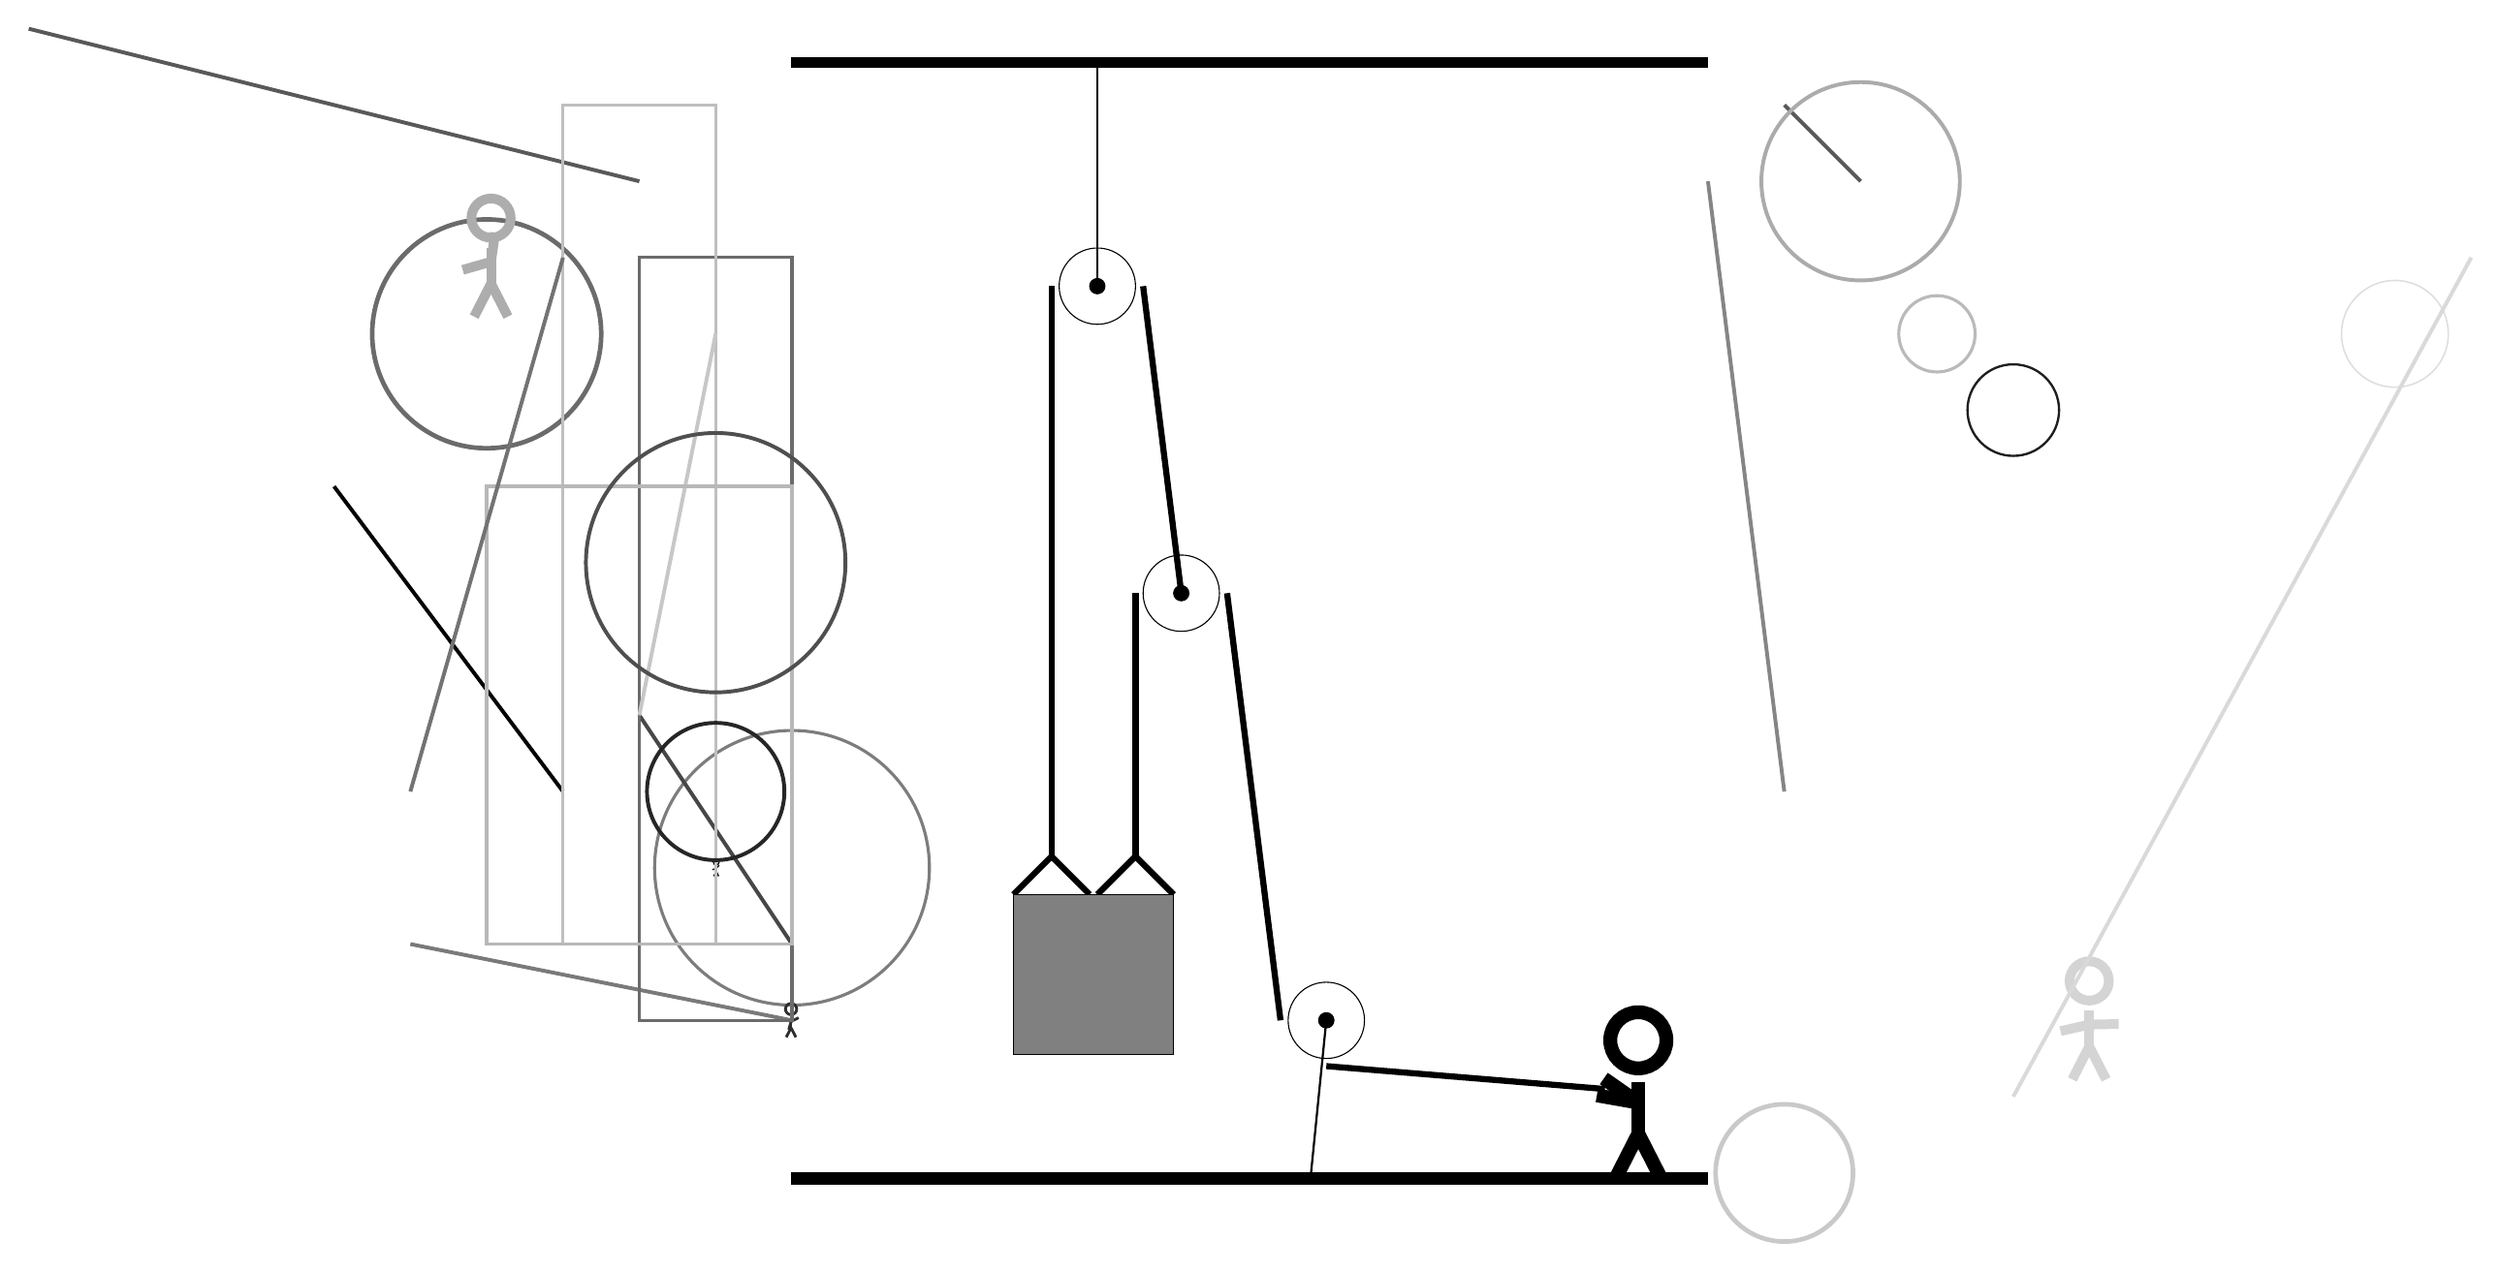
\begin{tikzpicture}
			%%%%% START %%%%%
			
			\draw[fill=black] (-2, 11.5) rectangle (10, 11.625);
			
			\draw (2, 8.625) circle (0.5);
			\draw[fill=black] (2, 8.625) circle (0.1);
			\draw[thick] (2, 8.625) -- (2, 11.5);
			
			\draw (3.1, 4.6) circle (0.5);
			\draw[fill=black] (3.1, 4.6) circle (0.1);
			
			\draw (5, -1) circle (0.5);
			\draw[fill=black] (5, -1) circle (0.1);
			\draw[thick] (5, -1) -- (4.8, -3);
			
			\draw[line width = 0.8mm]  (0.9, 0.65) -- (1.4, 1.15) -- (1.9, 0.65);
			\draw[line width = 0.8mm]  (2.0, 0.65) -- (2.5, 1.15) -- (3.0, 0.65);
			\draw[fill=black!50] (0.9, 0.65) rectangle (3.0, -1.45);
			
			\draw [line width=0.4mm, color=black!51](-2, 1) circle (1.8);
			
			\draw[line width=0.5mm, color=black!99](-5, 2) -- (-8, 6);
			\draw [line width=0.6mm, color=black!58](-6, 8) circle (1.5);
			\node[line width=0.3mm, color=black!82] at (-2, -1) {\Strichmaxerl[2][74][27]};
			
			\draw [line width=0.4mm, color=black!27](13, 8) circle (0.5);
			\draw[line width=0.5mm, color=black!65](11, 11) -- (12, 10);
			\draw[line width=0.5mm, color=black!52](-7, 0) -- (-2, -1);
			
			\draw[line width=0.5mm, color=black!72](-4, 3) -- (-2, 0);
			\draw[line width=0.5mm, color=black!48](11, 2) -- (10, 10);
			\draw[line width=0.5mm, color=black!65](-4, 10) -- (-12, 12);
			\draw[line width=0.4mm, color=black!58] (-4, -1) rectangle (-2, 9);
			
			\node[line width=0.3mm, color=black!17] at (15, -1) {\Strichmaxerl[7][13][1]};
			\draw [line width=0.3mm, color=black!88](14, 7) circle (0.6);
			
			\draw [line width=0.6mm, color=black!21](11, -3) circle (0.9);
			\node[line width=0.2mm, color=black!92] at (-3, 1) {\Strichmaxerl[1][18][47]};
			\draw[line width=0.4mm, color=black!25] (-3, 0) rectangle (-5, 11);
			
			\node[line width=0.7mm, color=black!32] at (-6, 9) {\Strichmaxerl[7][16][82]};
			\draw [line width=0.2mm, color=black!13](19, 8) circle (0.7);
			\draw[line width=0.5mm, color=black!15](14, -2) -- (20, 9);
			
			\draw[line width=0.5mm, color=black!22](-3, 8) -- (-4, 3);
			\draw[line width=0.5mm, color=black!28] (-2, 6) rectangle (-6, 0);
			
			\draw [line width=0.5mm, color=black!69](-3, 5) circle (1.7);
			
			\draw [line width=0.5mm, color=black!85](-3, 2) circle (0.9);
			\draw[line width=0.5mm, color=black!55](-7, 2) -- (-5, 9);
			\draw [line width=0.5mm, color=black!33](12, 10) circle (1.3);
			
			\draw[line width = 0.8mm] (1.4, 8.625) -- (1.4, 1.15);
			\centerarc[line width = 0.8mm](2, 8.625)(0:180:0.6);
			\draw[line width = 0.8mm] (2.6, 8.625) -- (3.1, 4.6);
			\draw[line width = 0.8mm] (2.5, 4.6) -- (2.5, 1.15);
			\centerarc[line width = 0.8mm](3.1, 4.6)(0:180:0.6);
			\draw[line width = 0.8mm] (3.7, 4.6) -- (4.4, -1);
			\centerarc[line width = 0.8mm](5, -1)(180:270:0.6);
			\draw[line width = 0.8mm] (5, -1.6) -- (8.65, -1.9);
			
			\node at (9, -2) {\Strichmaxerl[10][-35][170]};
			
			\draw[fill=black] (-2, -3) rectangle (10, -3.15);
			
			%%%%% END %%%%%
		\end{tikzpicture}
	\end{figure}	
\end{document}